\documentclass{article}
\usepackage[margin=1in]{geometry}
\usepackage{natbib}
\usepackage{changepage}
\usepackage[utf8]{inputenc} % allow utf-8 input
\usepackage[T1]{fontenc}    % use 8-bit T1 fonts
\usepackage{graphicx}
\usepackage{amsmath}
\usepackage{amsfonts}       % blackboard math symbols
\usepackage{hyperref}       % hyperlinks
\usepackage{cleveref}
\usepackage{url}            % simple URL typesetting
\usepackage{booktabs}       % professional-quality tables
\usepackage{nicefrac}       % compact symbols for 1/2, etc.
\usepackage{microtype}      % microtypography
\usepackage{xcolor}         % colors
\usepackage{tikz}
\usepackage{pgfplots}
\usepackage{float}
\pgfplotsset{compat=1.18}
\usepackage{authblk}
\usepackage{subcaption} 
\newcommand{\model}{GPT-NeoX-20B}
\newcommand{\stb}[1]{\textcolor{red}{#1}} 
\newcommand{\srb}[1]{\textcolor{blue}{#1}} 
\newcommand*{\tokenbox}[1]{\framebox{\strut #1}}
\usepackage{todonotes}

\DeclareMathOperator{\softmax}{softmax}


\title{\model: An Open-Source Autoregressive Language Model}

% The \author macro works with any number of authors. There are two commands
% used to separate the names and addresses of multiple authors: \And and \AND.
%
% Using \And between authors leaves it to LaTeX to determine where to break the
% lines. Using \AND forces a line break at that point. So, if LaTeX puts 3 of 4
% authors names on the first line, and the last on the second line, try using
% \AND instead of \And before the third author name.

% \mbox makes sure names arent broken in the middle
\renewcommand{\thefootnote}{\fnsymbol{footnote}} % Temporarily switch footnotes to symbols.
\author{\mbox{Sid Black\footnote{Authors after the first three are listed in alphabetical order. See \Cref{app:contrib} for individual contribution details.}}}
\author{\mbox{Stella Biderman\protect\footnotemark[1]}}
\author{\mbox{Eric Hallahan\protect\footnotemark[1]}}
\author{\authorcr\mbox{Quentin Anthony}}
\author{\mbox{Leo Gao}}
\author{\mbox{Laurence Golding}}
\author{\mbox{Horace He}}
\author{\mbox{Connor Leahy}}
\author{\mbox{Kyle McDonell}}
\author{\mbox{Jason Phang}}
\author{\mbox{Michael Pieler}}
\author{\mbox{USVSN Sai Prashanth}}
\author{\mbox{Shivanshu Purohit}}
\author{\mbox{Laria Reynolds}}
\author{\mbox{Jonathan Tow}}
\author{\mbox{Ben Wang}}
\author{\mbox{Samuel Weinbach}}
\affil{EleutherAI}
\date{} % hide date
\renewcommand{\thefootnote}{\arabic{footnote}} % Bring back Arabic footnotes.
\begin{document}

\maketitle

% not using \model in the abstract because it makes copypasting harded
\begin{abstract}

    GPT-NeoX-20B is a 20 billion parameter autoregressive language model whose weights will be made freely and openly available to the public through a permissive license. It is, to the best of our knowledge, the largest dense autoregressive model that has publicly available weights. In this paper, we describe the model architecture and training, evaluate its performance, and discuss the broader impacts of its release. We are open-sourcing the training and evaluation code, as well as the model weights, at \url{https://github.com/EleutherAI/gpt-neox}.
\end{abstract}

\section{Introduction}\label{sec:intro}

Over the past several years there has been an explosion in research surrounding large language models (LLMs) for natural language processing, catalyzed largely by the impressive performance of transformer based language models like BERT \citep{bert}, GPT-2 \citep{radford2019language}, GPT-3 \citep{brown2020language}, and T5 \citep{t5}. One of the most impactful outcomes of this research has been the finding that the performance of LLMs scales predictably as a power-law with the number of parameters, with architecture details such as width/depth ratio having a minimal effect within a wide range \citep{kaplan2020scaling}. A consequence of this has been an abundance of research focusing on scaling transformer models up to never before seen scales, resulting in models of up to 530B parameters \citep{megatron-530b}, a scale that would have been almost unthinkable just a few years prior.

Today, there are dozens of publicly acknowledged LLMs in existence. The largest have more than two orders of magnitude more parameters than GPT-2, and even at that scale there are nearly a dozen different models. However, these models are almost universally the protected intellectual property of large tech companies, and are gated behind a commercial API, available only upon request, or not available for outsider use at all. To our knowledge, the only freely and publicly available dense autoregressive language models larger than GPT-2 are GPT-Neo (2.7B parameters) \citep{black2021gpt}, GPT-J-6B \citep{gpt-j}, Megatron-11B\footnote{\url{https://github.com/pytorch/fairseq/tree/main/examples/megatron_11b}}, Pangu-$\alpha$-13B \citep{pangu}, and the recently released Fairseq 6.7 and 13B \citep{fairseq-13B} models.

Our release of \model{} is motivated by the belief that open access to LLMs is critical to advancing research in a wide range of areas---particularly in AI safety, mechanistic interpretability, and the study of how LLM capabilities scale. Many of the most interesting capabilities of LLMs only emerge above a certain number of parameters, and they have many properties that simply cannot be studied in smaller models. Although safety is often cited as a justification for keeping model weights private, we believe this is insufficient to prevent misuse, and is largely a limitation on the ability to probe and study LLMs for researchers not based at the small number of organizations that have access to state of the art language models.

\section{Model and Training Details}
\label{sec:model-details}

Our model architecture largely follows that of GPT-3 \citep{brown2020language}, with a few notable deviations described below. As our model size does not correspond to any of the models in \citet{brown2020language}, we interpolate between the hyperparameters they report to determine the values to use.

A link to download the weights of the model for checkpoints saved at evenly spaced 1000 step intervals throughout the whole training run will be released at \url{https://github.com/EleutherAI/gpt-neox}. We hope that making a wide range of checkpoints throughout training freely available will facilitate research into the training dynamics of LLMs, as well as being impactful in the aforementioned areas of AI safety and interpretability.

\begin{table*}[ht]
	\centering
	\begin{tabular}{rcccccc}
	    Params & Scaling & Layers & Model Dim & Heads & Batch Size & Learning Rate\\\midrule
	     20 B & 19.9 B & 44 & 6144 & 64 & 3.1 M & $9.7\times 10^{-5}$\\
	\end{tabular}
	\caption{``Params'' refers to all parameters while ``Scaling'' refers to \textit{non-embedding} parameters and should be the parameter count used for scaling laws research. Batch size is presented in tokens rather than the number of contexts, following \citet{brown2020language}. For a full list of hyperparameters and exact model sizes, see \Cref{app:hparam}.}
	\label{table:interp}
\end{table*}

\subsection{Model Architecture}
\label{sec:model-arch}

Although our architecture is largely similar to GPT-3, there are some notable differences. In this section we give a high-level overview of those differences, assuming the reader is familiar with the architecture of GPT-3. 

\paragraph{3D Parallelism} Since the weights and optimizer states of a model at this scale do not fit on a single GPU, we use the tensor parallelism scheme introduced in \citet{shoeybi2019megatron} in combination with pipeline parallelism to distribute the model across GPUs. To train \model{}, we found the most efficient way to distribute the model given our hardware setup to be a tensor parallel size of 2, and a pipeline parallel size of 4---allowing the most communication intensive processes, tensor and pipeline parallelism, to occur within a node, and data parallel communication to occur across node boundaries. It is assumed, although not detailed in the paper, that GPT-3 uses a similar scheme for parallelization.

\paragraph{Rotary Embeddings} Following on from our previous positive experiences \citep{rope-eleutherai,rope-experiments,gpt-j}, we use rotary embeddings \citep{su2021roformer} instead of the learned positional embeddings that OpenAI's GPT models use \citep{radford2018improving}. Rotary embeddings are a form of static relative positional embeddings that modify the attention equation to
$$\softmax\left(\frac{1}{\sqrt{d}}\sum_{n,m}\mathbf{x}_m^T\mathbf{W}^T_qR^{d}_{\Theta,(n-m)}\mathbf{W}_k\mathbf{x}_n\right),$$
where $R^d_{\Theta,x}$ is a $d\times d$ block diagonal matrix with the $i$th block being a $2$D rotation by $x\theta_i$ for hyperparameters $$\Theta = \{\theta_i = 10000^{-2(i-1)/d}\;\vert\;i\in\{0,1,2,\ldots, (d-1)/2\}\}.$$

While \citet{su2021roformer} applies rotary embeddings to every embedding vector, we follow \citet{gpt-j} and instead apply it only to the first $25\%$ of embedding vectors. Our experiments indicate that this strikes the best balance of performance and computational efficiency.\footnote{See the WandB reports \href{https://wandb.ai/eleutherai/neox/reports/Partial-Rotary-Tests-v2--Vmlldzo2MjE4MTQ}{here} and \href{https://wandb.ai/lucidrains/x-transformers-experiments/reports/partial-rotary--Vmlldzo2MjAyODY?accessToken=f657029yibaln2vseli6egxxwykhpeuedeuvcnmmdgn4i6d5b1r30it3mp0gw0k5}{here} for further details.}

\begin{figure}[h]
    \centering
    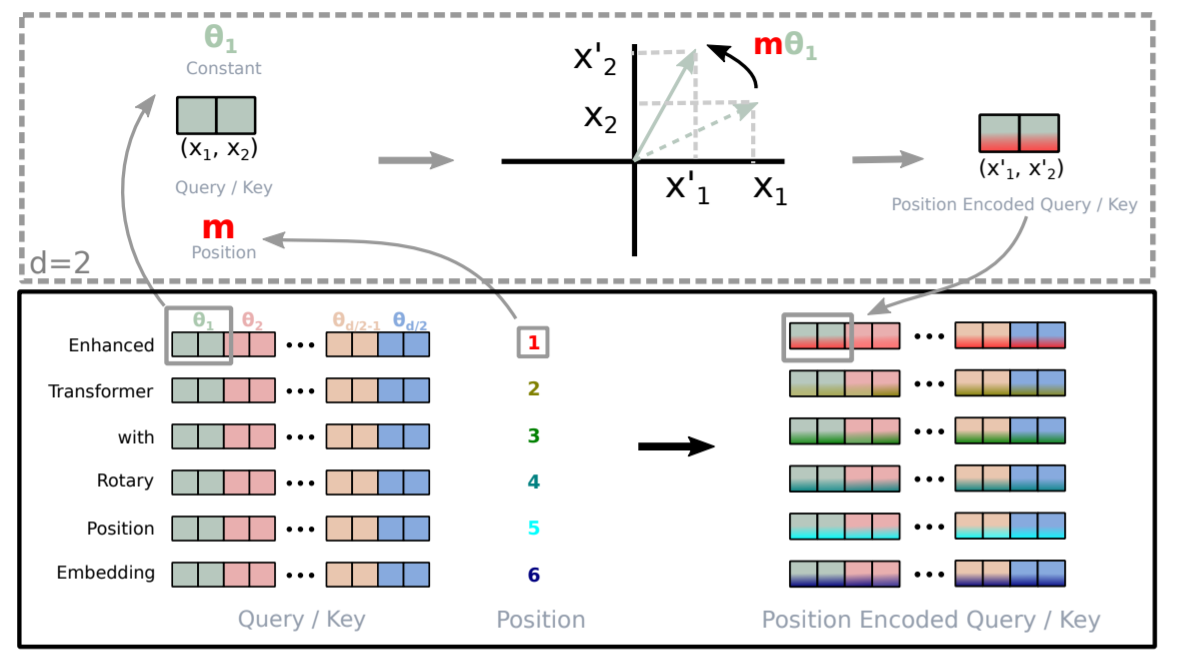
\includegraphics[width=0.75\textwidth]{Figures/rotary_diagram.png}
    \caption{A pictorial representation of rotary embeddings, from \citet{su2021roformer}.}
    \label{fig:my_label}
\end{figure}

\paragraph{Parallel Attention + FF Layers} As in \citet{mesh-transformer-jax}, we compute the Attention and Feed-Forward (FF) layers in parallel and add the results, rather than running them in series. This is primarily for efficiency purposes, as each residual addition with op-sharding requires one all-reduce in the forward pass and one in the backwards pass \citep{shoeybi2019megatron}. By computing the Attention and FFs in parallel, the results can be reduced locally before performing a single all-reduce. In Mesh Transformer JAX \citep{gpt-j}, this led to a 15\% throughput increase, while having comparable loss curves with running them in series during early training.

\paragraph{Initialization} 

For the Feed-Forward output layers before the residuals, we used the initialization scheme introduced in \citet{mesh-transformer-jax},

$$\frac{2}{L\sqrt{d}}$$

This prevents activations from growing with increasing depth and width, with the factor of 2 compensating for the fact that the parallel and feed-forward layers are organized in parallel. 

For all other layers, we use the \textit{small init} scheme from \citet{transformers-without-tears},

$$\sqrt{\frac{2}{d+4d}}$$

\paragraph{All Dense Layers} While GPT-3 alternates between dense and sparse layers using the technique introduced in \citet{child2019generating}, we instead opt to exclusively use dense layers to reduce implementation complexity.

\subsection{Training Hyperparameters}

Due to the intractability of performing a hyperparameter sweep for a 20 billion parameter model, we opted to use the values from \citet{brown2020language} to guide our choice of hyperparameters. As \citet{brown2020language} did not train a model at our exact scale, we interpolate between the learning rates of their 13B and 175B models to arrive at a learning rate of $0.97\mathrm{e}{-5}$. Based on the results of smaller scale experiments, we select a weight decay of 0.01. To achieve a higher training throughput, we opt to use the same batch size as OpenAI's 175B model--approximately 3.15M tokens, or 1538 contexts of 2048 tokens each, and train for a total of $150,000$ steps, decaying the learning rate with a cosine schedule to $10\%$ of its original value at the end of training.

We use the AdamW \citep{adamw} optimizer, with beta values of $0.9$ and $0.95$ respectively, and an epsilon of $1.0\mathrm{e}{-8}$. We extend AdamW with the \textit{ZeRO} optimizer \citep{zero} to reduce memory consumption by distributing optimizer states across ranks.

\subsection{Training Data}
\label{sec:training-data}

As the training data for GPT-3 was never publicly released, it was necessary to create our own training dataset which we call the Pile \citep{gao2020pile}. The Pile is a massive curated dataset that we designed specifically for training large language models. It consists of data from 22 data sources, coarsely broken down into 5 categories:

\begin{itemize}
    \item \textbf{Academic Writing}: Pubmed Abstracts and PubMed Central, arXiv, FreeLaw,\footnote{\url{https://www.courtlistener.com/}} USPTO Backgrounds,\footnote{\url{https://bulkdata.uspto.gov/}} PhilPapers,\footnote{\url{https://philpapers.org/}} NIH Exporter\footnote{\url{https://exporter.nih.gov/}}
    \item \textbf{Web-scrapes and Internet Resources}: CommonCrawl, OpenWebText2, StackExchange,\footnote{\url{https://archive.org/details/stackexchange}} Wikipedia (English)
    \item \textbf{Prose}: BookCorpus2, Bibliotik, Project Gutenberg \citep[PG-19;][]{raecompressive2019}
    \item \textbf{Dialogue}: Youtube subtitles, Ubuntu IRC,\footnote{\url{https://irclogs.ubuntu.com/}} OpenSubtitles \citep{lison-tiedemann-2016-opensubtitles2016}, Hacker News,\footnote{\url{https://news.ycombinator.com/}} EuroParl \citep{koehn-2005-europarl}
    \item \textbf{Miscellaneous}: GitHub, the DeepMind Mathematics dataset \citep{DBLP:journals/corr/abs-1904-01557}, Enron Emails \citep{10.1007/978-3-540-30115-8_22}
\end{itemize}

In aggregate, the Pile consists of over 825GiB of raw text data. The diverse data sources reflects our desire for a general-purpose language model. Certain compnents are up-sampled to obtain a more balanced data distribution. In contrast, GPT-3's training data consists of web-scrapes, books datasets, and Wikipedia. When comparing results in this work to GPT-3, the training data is almost certainly the biggest known unknown factor. Full details of the Pile can be found in our technical report \citep{gao2020pile} and the associated datasheet \citep{biderman2022datasheet}.

It is particularly notable that the Pile contains a scrape of StackExchange preprocessed into a Q/A form. Recent work \citep{biderman2022neural} has shown that this formulation heavily influences code generation, with prompts such as ``write a Java program that accepts 10 integers and shows them in reversed order.'' producing not only a code solution but also a natural language discussion of that code, as one might see on Stack Exchange.

\subsection{Hardware}
\todo[inline]{Need confirmation/clarification on exact details. -- Eric}
\begin{figure}[h]
    \centering
    %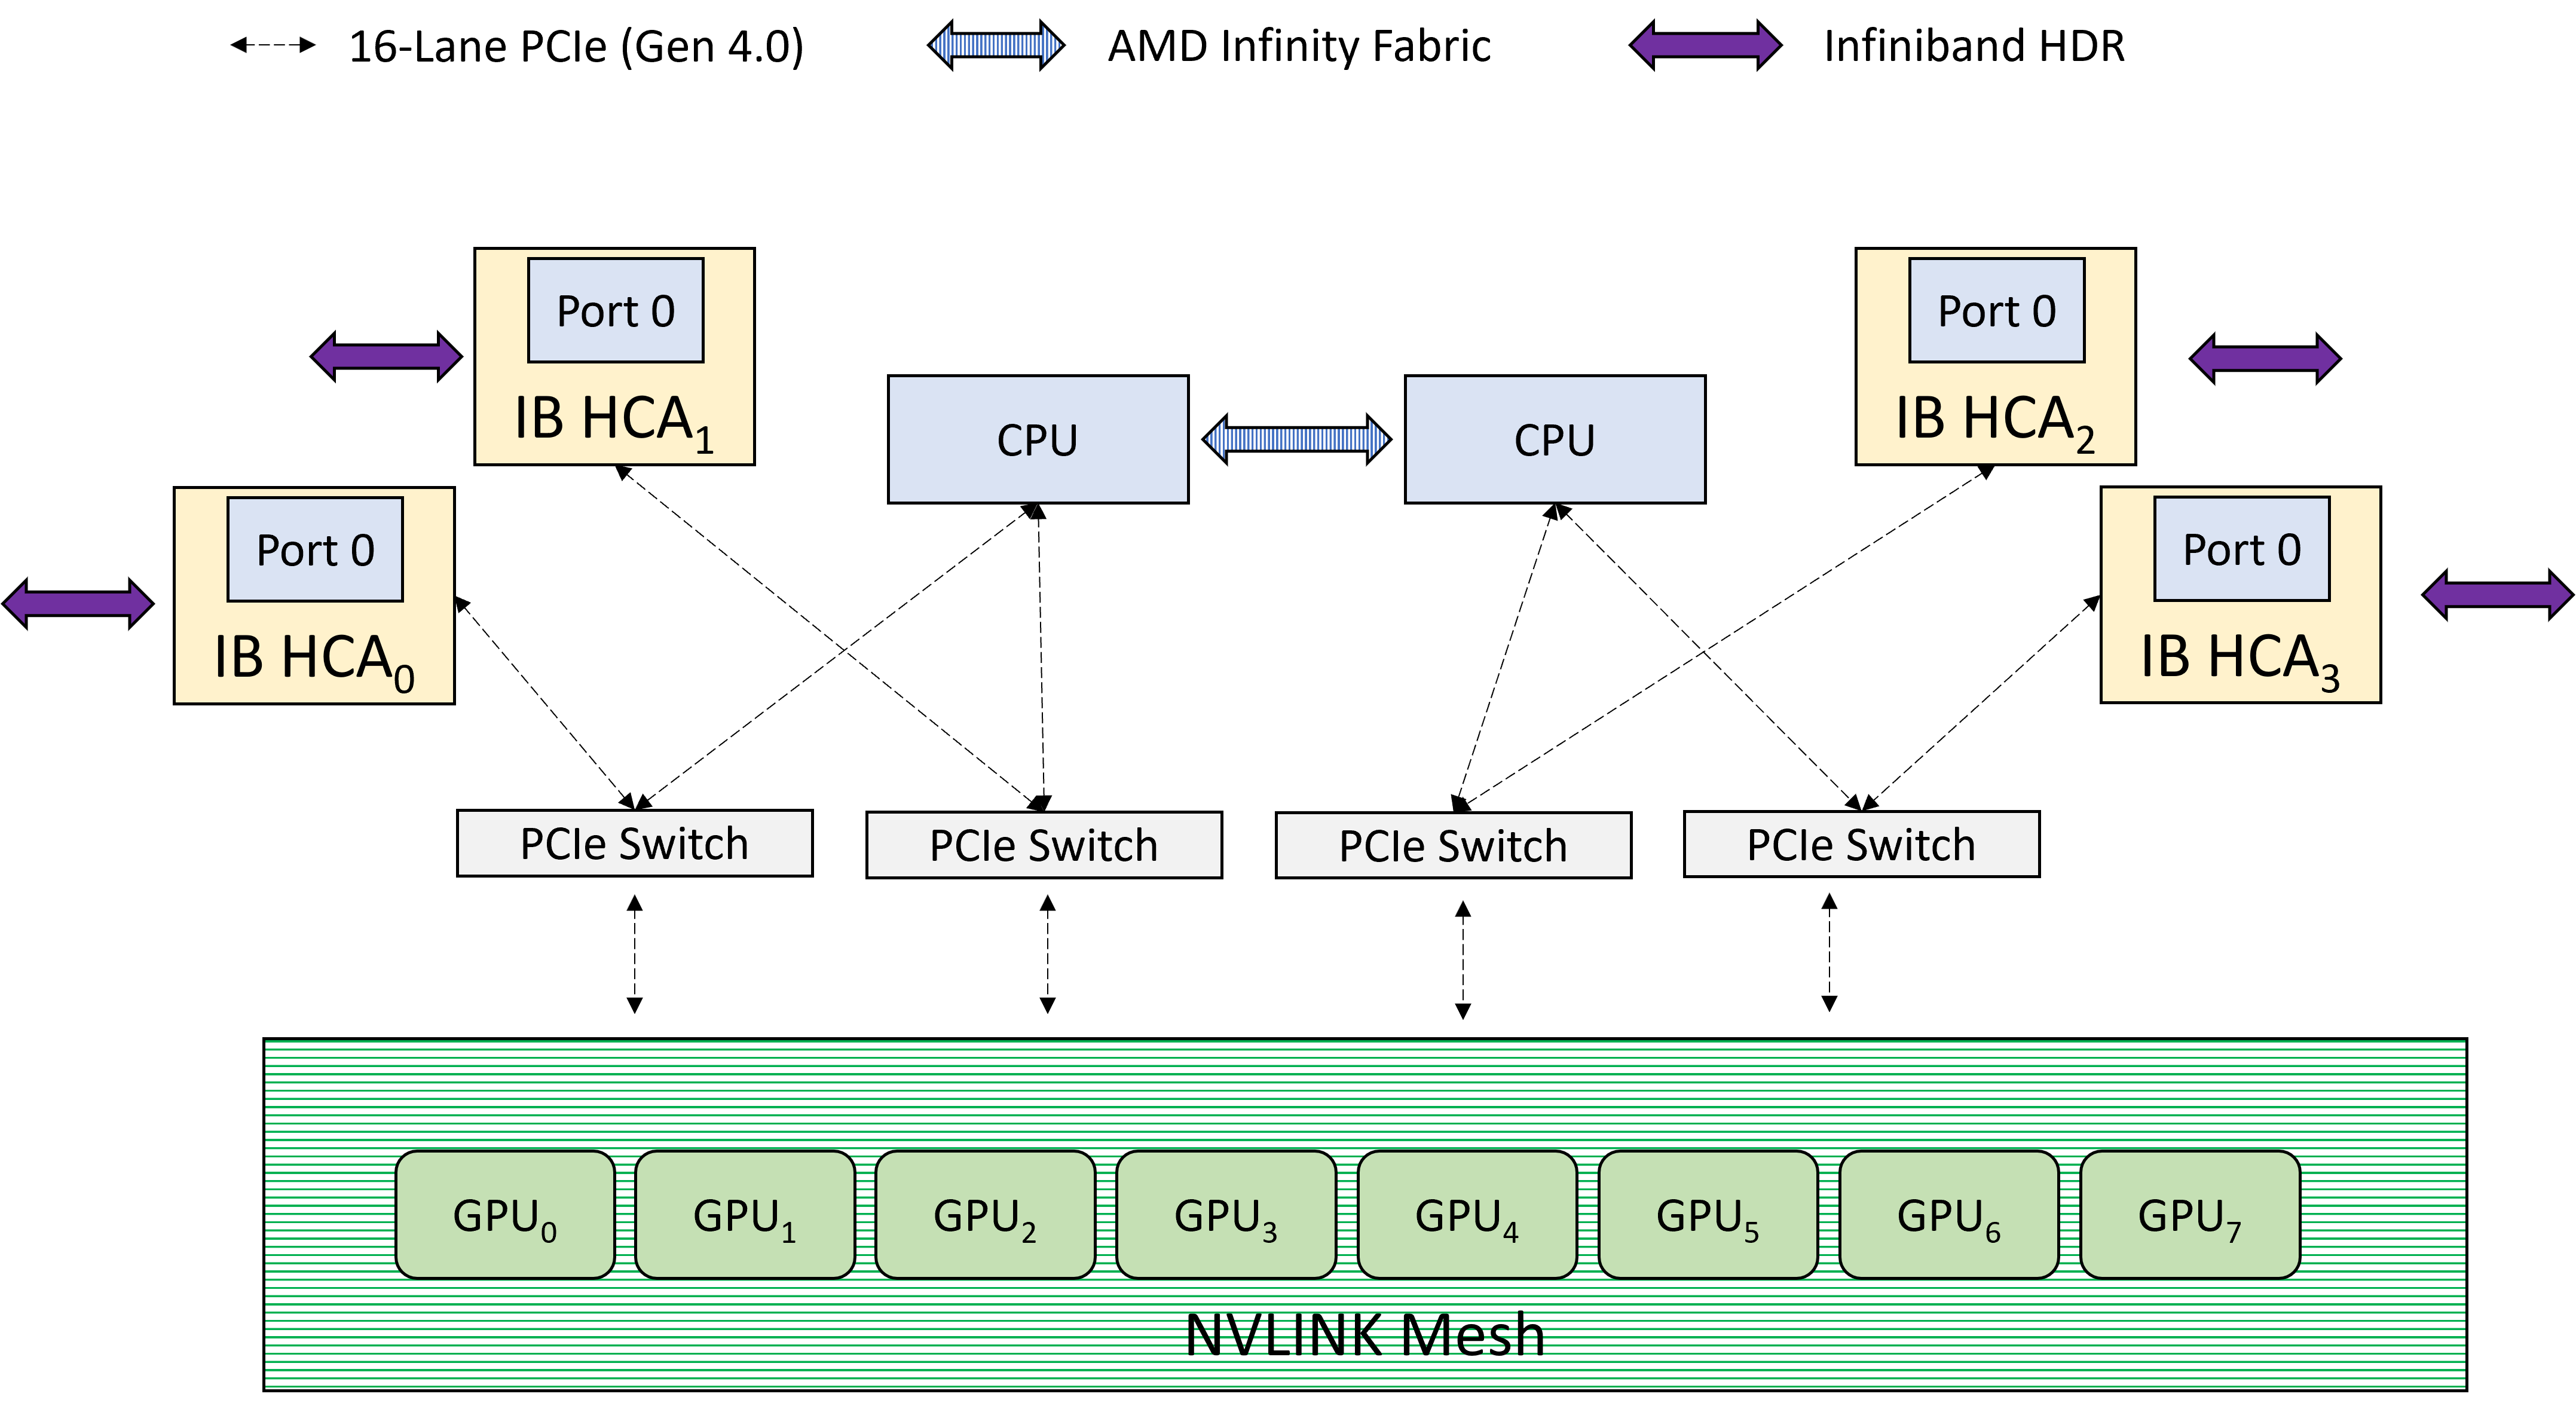
\includegraphics[width=0.75\textwidth]{Figures/neox-arch-placeholder.png}
    \usetikzlibrary{graphs,arrows.meta,calc}
\begin{tikzpicture}[new set=cpus,new set=plxs,new set=hcas,new set=gpus,new set=nvls]
	\begin{scope}[nodes=draw,align=center,shape=rectangle]
		\draw (0,0) foreach \cpui/\poscpu in {0/left,1/right} {
			+(\poscpu:0.25*\textwidth) node[set=cpus,minimum width=03/16*\textwidth,fill=blue!30](cpu\cpui) {\Large CPU{$_\cpui$}} 
			child[edge from parent/.style={draw=none},level distance=0.625in,sibling distance=0.125*\textwidth] foreach \plxi in {0,1} {
				node[set=plxs,fill=gray!30](plx\cpui\plxi) {\large PLX}
			}
		};
		\draw foreach \cpui/\plxi/\pos/\hcai in {0/0/left/0,0/1/right/1,1/0/left/2,1/1/right/3} {
			({plx\cpui\plxi}.south) ++(0,-0.125in) ++(\pos:0.125*\textwidth) node[set=hcas,fill=orange!30](hca\cpui\plxi) {\large HCA{$_\hcai$}}
		};
		\draw (-0.4375*\textwidth,-1.5in) foreach \gpui in {0,...,7} {
			+(\gpui*0.125*\textwidth,0)node[set=gpus,fill=green!30](gpu\gpui) {\large GPU{$_\gpui$}}
		};
		\foreach \gpui/\alias in {0/gpu000,1/gpu001,2/gpu011,3/gpu010,4/gpu100,5/gpu101,6/gpu111,7/gpu110}
			\pgfnodealias{\alias}{gpu\gpui};
		\draw (-0.416666667*\textwidth,-2.125in) foreach \nvli in {0,...,5} {
			+(\nvli*0.166666667*\textwidth,0) node[set=nvls,fill=green!50!gray!30](nvl\nvli) {NVSwitch{$_\nvli$}}
		};
	\end{scope}
	\begin{scope}[infiniband/.style={color=violet,arrows={{Triangle[]}-{Triangle[]}},thick,auto},pciexpress/.style={arrows={{Latex[]}-{Latex[]}},auto},xgmi2/.style={color=blue!50!black,arrows={{Latex[]}-{Latex[]}},auto},nvlink/.style={color=green!50!black,line cap=round}]
		\foreach \gpui[count=\gpuj] in {0,...,7}
			\foreach \nvli[count=\nvlj] in {0,...,5}
				\draw[nvlink] ($ ({gpu\gpui}.south west)!\nvlj/7!({gpu\gpui}.south east) + (0,-0.2pt)$) to node(nvlink\gpui\nvli) {} ($ ({nvl\nvli}.north west)!\gpuj/9!({nvl\nvli}.north east) + (0,+0.2pt)$);
		\draw[nvlink,right] (nvlink00) node[right](nvlinktext) {\footnotesize 2x};
		\begin{scope}[pciexpress]
			\foreach \cpui in {0,1}
				\foreach \plxi/\pos/\posi in {0/west/east,1/east/west}
					\draw ($ ({cpu\cpui}.south)!1/3!({cpu\cpui}.south \pos)$) --  +(0,-0.2in) -| node[anchor=\posi]{\footnotesize 16x} ({plx\cpui\plxi}.north);
			\foreach \cpui/\plxi/\pos in {0/0/east,0/1/west,1/0/east,1/1/west}
				\draw ($ ({plx\cpui\plxi}.south)!-1/2!({plx\cpui\plxi}.south \pos)$) |- node[ near end, below]{\footnotesize 16x} ({hca\cpui\plxi}.{\pos});
			\foreach \cpui/\plxi/\pos in {0/0/left,0/1/right,1/0/left,1/1/right}
				\draw[infiniband] ({hca\cpui\plxi}.north) -- node(ib\cpui\plxi){\footnotesize 4x} ++(0,0.375in) node[anchor=south](switch\cpui\plxi){\footnotesize Switch{$_\plxi$}};
			\foreach \cpui in {0,1}
				\foreach \plxi/\pos in {0/east,1/west}
					\draw ({plx\cpui\plxi}.south) -- ++(0,-0.375in) -| node[ near start, below]{\footnotesize 16x} ({gpu\cpui\plxi0}.north);
			\foreach \cpui in {0,1}
				\foreach \plxi/\pos/\posi in {0/east/west,1/west/east}
					\draw ($ ({plx\cpui\plxi}.south)!1/2!({plx\cpui\plxi}.south \pos)$) -- node[near end, anchor=\posi]{\footnotesize 16x} ++(0,-0.5in) -| ({gpu\cpui\plxi1}.north) ;
			\draw[xgmi2] ($ (cpu0.north east)!1/5!(cpu0.south east) $) -- node(xgmi) {\footnotesize 16x} ($ (cpu1.north west)!1/5!(cpu1.south west)$);%
			\foreach \xgmii in {2,...,4} 
			    \draw[xgmi2] ($ (cpu0.north east)!\xgmii/5!(cpu0.south east) $) -- node(xgmi\xgmii){} ($ (cpu1.north west)!\xgmii/5!(cpu1.south west) $);%xGMI-2
		\end{scope}
		\draw[infiniband] (-7/16*\textwidth,0.5in) -- +(1/16*\textwidth,0) node[yshift=0.125in](ib) {\small\strut HDR InfiniBand} node[yshift=-0.125in](ibspeed) {\scriptsize\strut 50 GT/s per lane} -- +(1/8*\textwidth,0);
		\draw[pciexpress] (-3/16*\textwidth,0.5in) -- +(1/16*\textwidth,0) node[centered,yshift=0.125in](pcie) {\small\strut PCI Express 4.0} node[yshift=-0.125in](pciespeed) {\scriptsize\strut 16 GT/s per lane} -- +(1/8*\textwidth,0);
		\draw[xgmi2] (1/16*\textwidth,0.5in) -- +(1/16*\textwidth,0) node[yshift=0.125in](xgmi) {\small\strut xGMI-2} node[yshift=-0.125in](xgmispeed) {\scriptsize\strut 16 GT/s per lane}
		-- +(1/8*\textwidth,0);%
		\draw[nvlink] (5/16*\textwidth,0.5in) -- +(1/16*\textwidth,0) node[yshift=0.125in](nvlink) {\small\strut NVLink 3.0} node[yshift=-0.125in](nvlinkspeed) {\scriptsize\strut 400 GT/s per lane}
		-- +(1/8*\textwidth,0);
	\end{scope}
\end{tikzpicture}
    \caption{Architecture diagram of a single training node.}
    \label{fig:training-node}
\end{figure}

We trained \model{} on twelve Supermicro AS-4124GO-NART servers, each with eight NVIDIA A100-SXM4-40GB GPUs and configured with two AMD EPYC 7532 CPUs. Figure~\ref{fig:training-node} shows a simplified overview of a node as configured for training.

% From TastyBucketOfRice: What does this sentence mean? "with two banks of six nodes ..."
As interconnect is the single most critical subsystem when training large models, each node is equipped with four HCAs connected to one of two NVIDIA MQM8700-HS2R switches to construct a distributed star topology with two stars of six nodes each. Due to supply constraints, a mixture of ConnectX-5 and ConnectX-6 HCAs fufilled this role.

\subsection{Software Libraries}

Our model is trained using a custom codebase that we call GPT-NeoX \citep{gpt-neox}. GPT-NeoX builds on Megatron \citep{shoeybi2019megatron} and DeepSpeed \citep{deepspeed} to facilitate efficient and straightforward training of large language models with tens of billions of parameters.

We use the official PyTorch v1.10.0 release binary package compiled with CUDA 11.1. This package is bundled with NCCL 2.10.3 for distributed communications.

All evaluations were performed on the EleutherAI Language Model Evaluation Harness \citep{eval-harness}.

\subsection{Tokenization}
\label{sec:tokenization}

For \model{}, we use a BPE-based tokenizer similar to that used in GPT-2, with the same total vocabulary size of 50257. We make three major changes to the tokenizer. First, we train a new BPE tokenizer based on the Pile, taking advantage of its diverse text sources to construct a more general-purpose tokenizer. Second, in contrast to the GPT-2 tokenizer which treats tokenization at the start of a string as a non-space-delimited token, the \model{} tokenizer applies consistent space delimitation regardless. This resolves an inconsistency regarding the presence of prefix spaces to a tokenization input.\footnote{\url{https://discuss.huggingface.co/t/bpe-tokenizers-and-spaces-before-words/475/2}} An example can be seen in Figure~\ref{fig:tok_example}.
Third, our tokenizer contains tokens for repeated space tokens (all positive real numbers of repeated spaces up to and including 24) and, in total allocates 284 tokens to different combinations of whitespace characters, compared to 7 tokens in GPT-2. This allows the \model{} tokenizer to tokenize text with large amounts of whitespace using fewer tokens; for instance, program source code or arXiv LaTeX source files.

\begin{figure}[h]
    \centering
    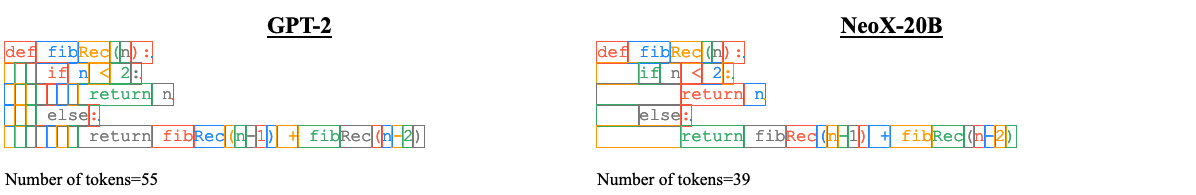
\includegraphics[width=0.95\textwidth]{Figures/tokenization/tokenization_example.png}
    \caption{GPT-2 tokenization vs. \model{} tokenization. \model{} tokenization handles whitespace better, which can be particularly useful for text such as source code.}
    \label{fig:tok_example}
\end{figure}


\subsubsection{Tokenizer Comparisons on Pretraining Corpora}

Both tokenizers share 36938 out of 50257 tokens, a $\sim$73.5\% overlap in tokens.
In this section, we perform comparison between the \model{} tokenizer to the GPT-2 tokenizer using the validation set of the Pile.

In Table~\ref{tab:token_pileval-all}, we show the resulting number of tokens from tokenizing each component of the Pile’s validation set with both tokenizers, and the ratio of \model{} tokens to GPT-2 tokens.


\begin{table}[ht!]
\centering
\begin{subtable}[h]{0.48\textwidth}
\resizebox{1\textwidth}{!}{
\begin{tabular}{lrrcc}
\toprule
    & GPT-2 & \model & $\frac{\text{\model}}{\text{GPT-2}}$ \\ 
    \midrule
    ArXiv & 41,020,155 & 34,704,315 & 0.84603 \\
    BookCorpus2 & 2,336,388 & 2,365,633 & 1.01252 \\
    Books3 & 42,819,036 & 43,076,832 & 1.00602 \\
    DM Mathematics & 7,699,527 & 7,413,775 & 0.96289 \\
    Enron Emails & 480,500 & 433,867 & 0.90295 \\
    EuroParl & 3,519,584 & 2,808,275 & 0.79790 \\
    FreeLaw & 21,098,168 & 18,687,364 & 0.88573 \\
    Github & 42,986,216 & 33,021,839 & 0.76820 \\
    Gutenberg (PG-19) & 6,729,187 & 6,428,946 & 0.95538 \\
    HackerNews & 2,578,933 & 2,551,720 & 0.98945 \\
    NIH ExPorter & 776,688 & 739,558 & 0.95219 \\
    OpenSubtitles & 5,431,529 & 5,446,485 & 1.00275 \\
    OpenWebText2 & 31,993,480 & 30,813,744 & 0.96313 \\
    PhilPapers & 1,879,206 & 1,750,928 & 0.93174 \\
    Pile-CC & 53,415,704 & 53,392,389 & 0.99956 \\
    PubMed Abstracts & 8,708,180 & 8,215,529 & 0.94343 \\
    PubMed Central & 56,874,247 & 43,534,166 & 0.76545 \\
    StackExchange & 22,708,643 & 19,000,198 & 0.83669 \\
    USPTO Backgrounds & 10,217,886 & 9,727,223 & 0.95198 \\
    Ubuntu IRC & 3,341,287 & 2,771,066 & 0.82934 \\
    Wikipedia (en) & 12,614,087 & 12,692,048 & 1.00618 \\
    YoutubeSubtitles & 3,883,103 & 3,311,907 & 0.85290 \\
    \midrule
    Total & 383,111,734 & 342,887,807 & 0.89501 \\
    \bottomrule
\end{tabular}
}
\caption{All tokens}
\label{tab:token_pileval-all}
\end{subtable}
\hfill
\begin{subtable}[h]{0.48\textwidth}
\resizebox{\textwidth}{!}{
\begin{tabular}{lrrcc}
\toprule
    & GPT-2 & \model & $\frac{\text{\model}}{\text{GPT-2}}$ \\ 
    \midrule
    ArXiv & 38,932,524 & 33,561,364 & 0.86204 \\
    BookCorpus2 & 2,233,367 & 2,262,609 & 1.01309 \\
    Books3 & 40,895,236 & 41,198,424 & 1.00741 \\
    DM Mathematics & 7,214,874 & 6,929,066 & 0.96039 \\
    Enron Emails & 374,978 & 373,498 & 0.99605 \\
    EuroParl & 3,482,120 & 2,780,405 & 0.79848 \\
    FreeLaw & 17,766,692 & 17,434,708 & 0.98131 \\
    Github & 29,338,176 & 27,558,966 & 0.93936 \\
    Gutenberg (PG-19) & 5,838,580 & 5,827,408 & 0.99809 \\
    HackerNews & 2,312,116 & 2,299,848 & 0.99469 \\
    NIH ExPorter & 776,619 & 739,543 & 0.95226 \\
    OpenSubtitles & 5,428,118 & 5,445,721 & 1.00324 \\
    OpenWebText2 & 30,849,218 & 29,723,143 & 0.96350 \\
    PhilPapers & 1,872,347 & 1,743,627 & 0.93125 \\
    Pile-CC & 51,305,080 & 51,281,909 & 0.99955 \\
    PubMed Abstracts & 8,676,790 & 8,185,417 & 0.94337 \\
    PubMed Central & 44,508,570 & 40,722,151 & 0.91493 \\
    StackExchange & 17,414,955 & 16,712,814 & 0.95968 \\
    USPTO Backgrounds & 9,882,473 & 9,601,385 & 0.97156 \\
    Ubuntu IRC & 3,220,797 & 2,659,225 & 0.82564 \\
    Wikipedia (en) & 11,874,878 & 11,986,567 & 1.00941 \\
    YoutubeSubtitles & 3,589,042 & 3,046,451 & 0.84882 \\
    \midrule
    Total & 337,787,550 & 322,074,249 & 0.95348 \\
    \bottomrule
\end{tabular}
}
\caption{Excluding whitespace tokens}
\label{tab:token_pileval-nowhitespace}
\end{subtable}
\caption{
    Number of tokens from tokenizing the Pile validation set. (a) shows the full token count, (b) exclude whitespace tokens
}
\label{tab:token_pileval}

\end{table}

We see that the \model{} tokenizer represents all Pile components using fewer or very closely comparable numbers of tokens. The largest percentage improvement in token counts are in the EuroParl, Github, and PubMed Central components, with a more than 20\% savings in the number of tokens needed to represent that component. We highlight that ArXiv, Github and StackExchange, components with large code components, can be represented with meaningfully fewer tokens with the \model{} tokenizer compared to the GPT-2 tokenizer. Overall, the \model{} tokenizer represents the Pile validation set with approximately 10\% fewer tokens compared to the GPT-2 tokenizer.

As our tokenizer is tweaked to better tokenize whitespace, we also perform a comparison between the two tokenizers excluding whitespace. We perform the same analysis as the above, but exclude all whitespace tokens from our computations, only counting the non-whitespace tokens. A token is considered a whitespace token if it consists only of whitespace characters. The results are shown in Table~\ref{tab:token_pileval-nowhitespace}. We observe that the \model{} tokenizer still uses 5\% fewer tokens to represent the Pile validation set compared to the GPT-2 tokenizer. As expected, the token ratios for certain components such as Github and StackExchange become closer to even once the whitespace characters are excluded. 

\begin{table}[ht!]
\centering
\resizebox{0.6\textwidth}{!}{
\begin{tabular}{lrrcc}
\toprule
    & GPT-2 & \model{} & $\frac{\text{\model}}{\text{GPT-2}}$ \\ 
    \midrule
    C4 Tokens & 173,669,294 & 173,768,876  & 1.00057 \\
    C4 Tokens excl. Space & 168,932,391 & 171,003,008 & 1.01226 \\
    \bottomrule
\end{tabular}
}
\caption{
    Number of tokens from tokenizing the AllenAI C4 (\texttt{en}) validation set.
}
\label{tab:token_c4}
\end{table}

Given that the \model{} is trained on the Pile, the Pile components would be considered in-domain for the tokenizer, and hence it may not provide the most informative comparison between the two. To perform an out-of-domain comparison, we perform the same analysis using the AllenAI replication of C4,\footnote{\url{https://github.com/allenai/allennlp/discussions/5056}}, another popular pretraining corpus for large language models. As above, we use the validation set for our analysis. Our results are shown in Table~\ref{tab:token_c4}. We find that the \model{} tokenizer tokenizes the C4 validation set to approximately the same number of tokens as the GPT-2 tokenizer. When excluding all whitespace tokens, the \model{} requires approximately 1\% more tokens to represent the corpus compared to the GPT-2 tokenizer. 

\subsubsection{In-Depth Comparison}

\paragraph{Tokenization Examples}

We show here several examples of the tokenization using both GPT-2 and \model{} tokenizers. More examples can be found in the appendix.

\paragraph{Longest Tokens}

We show in Table~\ref{tab:token_longest} the 10 longest tokens in each tokenizer vocabulary. We exclude consideration of tokens that comprise only symbols or whitespace characters. We observe that for the GPT-2 tokenizer, many of the longest tokens appear to reflect artifacts in the tokenizer training data, likely with certain websites or web-scrapes being overrepresented in the training data. For the \model{} tokenizer, we observe that most of the longest tokens are scientific terms, likely arising from the PubMed components of the Pile.

\begin{table}[ht!]
\centering
\resizebox{0.6\textwidth}{!}{
\begin{tabular}{lll}
\toprule
    & GPT-2 & \model  \\ 
    \midrule
    & \texttt{rawdownloadcloneembedreportprint} & \texttt{Ġimmunohistochemistry} \\
    & \texttt{BuyableInstoreAndOnline} & \texttt{Ġimmunohistochemical} \\
    & \texttt{cloneembedreportprint} & \texttt{Ġtelecommunications} \\
    & \texttt{ĠRandomRedditorWithNo} & \texttt{Ġimmunofluorescence} \\
    & \texttt{Ġtelecommunications} & \texttt{Ġimmunosuppressive} \\
    & \texttt{channelAvailability} & \texttt{ĠBytePtrFromString} \\
    & \texttt{Ġdisproportionately} & \texttt{Ġmultidisciplinary} \\
    & \texttt{ĠTelecommunications} & \texttt{Ġhistopathological} \\
    & \texttt{ĠguiActiveUnfocused} & \texttt{Ġneurodegenerative} \\
    & \texttt{ItemThumbnailImage} & \texttt{Ġindistinguishable} \\
    \bottomrule
\end{tabular}
}
\caption{
    Ten longest tokens (excluding tokens comprising mainly symbols, numbers and spaces) in tokenizer vocabularies. ``Ġ'' indicates a word delimiter.
}
\label{tab:token_longest}
\end{table}

\paragraph{Worst Case Word Tokenization Comparison}

\begin{table}[ht!]
\centering
\resizebox{\textwidth}{!}{
\begin{tabular}{lll}
\multicolumn{3}{c}{\large\textbf{GPT-2 Worst-case Tokenization}}\\
\toprule
    Word & GPT-2 Tokenization & \model{} Tokenization  \\ 
    \midrule
hematopoietic & (6) \texttt{\tokenbox{Ġhe}\tokenbox{mat}\tokenbox{op}\tokenbox{o}\tokenbox{iet}\tokenbox{ic}} &  (1) \texttt{\tokenbox{Ġhematopoietic}} \\
adenocarcinoma & (6) \texttt{\tokenbox{Ġad}\tokenbox{en}\tokenbox{oc}\tokenbox{arc}\tokenbox{in}\tokenbox{oma}} &  (1) \texttt{\tokenbox{Ġadenocarcinoma}} \\
MERCHANTABILITY & (5) \texttt{\tokenbox{ĠMER}\tokenbox{CH}\tokenbox{AN}\tokenbox{TA}\tokenbox{BILITY}} &  (1) \texttt{\tokenbox{ĠMERCHANTABILITY}} \\
CONSEQUENTIAL & (5) \texttt{\tokenbox{ĠCON}\tokenbox{SE}\tokenbox{QU}\tokenbox{ENT}\tokenbox{IAL}} &  (1) \texttt{\tokenbox{ĠCONSEQUENTIAL}} \\
oligonucleotides & (5) \texttt{\tokenbox{Ġolig}\tokenbox{on}\tokenbox{ucle}\tokenbox{ot}\tokenbox{ides}} &  (1) \texttt{\tokenbox{Ġoligonucleotides}} \\
cytoplasmic & (5) \texttt{\tokenbox{Ġcy}\tokenbox{top}\tokenbox{l}\tokenbox{asm}\tokenbox{ic}} &  (1) \texttt{\tokenbox{Ġcytoplasmic}} \\
corticosteroids & (4) \texttt{\tokenbox{Ġcort}\tokenbox{ic}\tokenbox{oster}\tokenbox{oids}} &  (1) \texttt{\tokenbox{Ġcorticosteroids}} \\
neurodegenerative & (4) \texttt{\tokenbox{Ġneuro}\tokenbox{deg}\tokenbox{ener}\tokenbox{ative}} &  (1) \texttt{\tokenbox{Ġneurodegenerative}} \\
asymptotic & (4) \texttt{\tokenbox{Ġas}\tokenbox{ym}\tokenbox{pt}\tokenbox{otic}} &  (1) \texttt{\tokenbox{Ġasymptotic}} \\
aneurysm & (4) \texttt{\tokenbox{Ġan}\tokenbox{eur}\tokenbox{ys}\tokenbox{m}} &  (1) \texttt{\tokenbox{Ġaneurysm}} \\
    \bottomrule
\end{tabular}
\bigskip
\begin{tabular}{lll}
\multicolumn{3}{c}{\large\textbf{\model{} Worst-case Tokenization}}\\
\toprule
    Word & GPT-2 Tokenization & \model{} Tokenization  \\ 
    \midrule
    Schwarzenegger & (1) \texttt{\tokenbox{ĠSchwarzenegger}} &  (5) \texttt{\tokenbox{ĠSch}\tokenbox{war}\tokenbox{zen}\tokenbox{eg}\tokenbox{ger}} \\
Bolshevik & (1) \texttt{\tokenbox{ĠBolshevik}} &  (4) \texttt{\tokenbox{ĠB}\tokenbox{ols}\tokenbox{he}\tokenbox{vik}} \\
crowdfunding & (1) \texttt{\tokenbox{Ġcrowdfunding}} &  (4) \texttt{\tokenbox{Ġcrow}\tokenbox{df}\tokenbox{und}\tokenbox{ing}} \\
misogyny & (1) \texttt{\tokenbox{Ġmisogyny}} &  (4) \texttt{\tokenbox{Ġmis}\tokenbox{og}\tokenbox{yn}\tokenbox{y}} \\
McAuliffe & (1) \texttt{\tokenbox{ĠMcAuliffe}} &  (4) \texttt{\tokenbox{ĠMc}\tokenbox{A}\tokenbox{ul}\tokenbox{iffe}} \\
unstoppable & (1) \texttt{\tokenbox{Ġunstoppable}} &  (4) \texttt{\tokenbox{Ġun}\tokenbox{st}\tokenbox{opp}\tokenbox{able}} \\
Timberwolves & (1) \texttt{\tokenbox{ĠTimberwolves}} &  (4) \texttt{\tokenbox{ĠTim}\tokenbox{ber}\tokenbox{w}\tokenbox{olves}} \\
excruciating & (1) \texttt{\tokenbox{Ġexcruciating}} &  (4) \texttt{\tokenbox{Ġexc}\tokenbox{ru}\tokenbox{ci}\tokenbox{ating}} \\
Kaepernick & (1) \texttt{\tokenbox{ĠKaepernick}} &  (4) \texttt{\tokenbox{ĠK}\tokenbox{ae}\tokenbox{per}\tokenbox{nick}} \\
Valkyrie & (1) \texttt{\tokenbox{ĠValkyrie}} &  (4) \texttt{\tokenbox{ĠV}\tokenbox{alk}\tokenbox{y}\tokenbox{rie}} \\
    \bottomrule
\end{tabular}
}
\caption{
  Worst case word tokenization with respective tokenizers. 
  We show cases where one tokenizer requires many more tokens to represent a word compared to the other tokenizer. 
  The worst case tokenization for GPT-2 is shown on the left, and \model{} on the right.
  ``Ġ'' indicates a word delimiter.
}
\label{tab:token_worst}
\end{table}

We consider the words for which there is the greatest discrepancy in the resulting token length between the two tokenizers, where one tokenizer needs many tokens to represent while the other tokenizer uses relatively few tokens. We define a word as a contiguous string delimited by whitespace or punctuation (as defined by \texttt{strings.punctuation} in Python). We perform this analysis at the component level. We only consider words that occur at least 10 times within the given component. We show in Table~\ref{tab:token_worst} a representative example from the Pile-CC corpus.

\section{Performance Evaluations}
\label{sec:evals}

To evaluate our model we use \citet{eval-harness}, an open source codebase for language model evaluation that supports a number of model APIs. We compare with the GPT-3 API \citep{brown2020language}
\footnote{The numbers do not always agree with the numbers reported in \citet{brown2020language}, because our prompt formatting is slightly different from theirs.}, the open source FairSeq dense models \citep{fairseq-13B}, and GPT-J \citep{gpt-j}. We do not compare against T5 \citep{t5} as our evaluation methodology assumes the models are autoregressive, or T0 \citep{sanh2021multitask} because the T0 API does not allow for computing log-likelihoods.

When we were able to obtain the relevant information, we report two baselines: human level performance and random performance.

\subsection{Performance Across Training}

\todo[inline]{Guac has a bunch of evals on partially trained models saved at \texttt{/mnt/ssd-1/20B\_eval\_results/iteration\_}. These need to be plotted and put here.}

\subsection{Natural Language Tasks}
\todo[inline]{pls include task versions in all performance tables!!! -leo}
\begin{table}[ht!]
\centering
\resizebox{\textwidth}{!}{
\begin{tabular}{lcccccccc}
\toprule
            & Version & Babbage    & GPT-J & FairSeq 6.7B & Curie & FairSeq 13B & GPT-NeoX 20B & DaVinci\\\midrule
ANLI R1     & 0 & Babfbage    & GPT-J & FairSeq 6.7B & Curie & FairSeq 13B & GPT-NeoX 20B & DaVinci\\ 
ANLI R2     & 0 & Babbage    & GPT-J & FairSeq 6.7B & Curie & FairSeq 13B & GPT-NeoX 20B & DaVinci\\ 
ANLI R3     & 0 & Babbage    & GPT-J & FairSeq 6.7B & Curie & FairSeq 13B & GPT-NeoX 20B & DaVinci\\ 
HellaSwag   & 0 & Babbage    & GPT-J & FairSeq 6.7B & Curie & FairSeq 13B & GPT-NeoX 20B & DaVinci\\ 
LAMBADA     & 0 & Babbage    & GPT-J & FairSeq 6.7B & Curie & FairSeq 13B & GPT-NeoX 20B & DaVinci\\ 
WSC         & 0 & Babbage    & GPT-J & FairSeq 6.7B & Curie & FairSeq 13B & GPT-NeoX 20B & DaVinci\\ 
Winogrande  & 0 & Babbage    & GPT-J & FairSeq 6.7B & Curie & FairSeq 13B & GPT-NeoX 20B & DaVinci\\ 
    \midrule
    \bottomrule
\end{tabular}
}
\caption{
    placeholder
}
\label{tab:nl_evals}
\end{table}

\subsection{Knowledge-Based Tasks}

In addition to evaluating on natural language processing benchmarks, we are also interested in the ability of our models to answer factual questions requiring advanced knowledge. To do this, we use a dataset of multiple choice questions in a variety of diverse domains developed by \citet{hendrycks2020measuring}. As individual subjects are rather noisy, we follow \citep{hendrycks2020measuring} by focusing on results aggregated by subject area: Humanities, Social Sciences, STEM, and Miscellaneous as presented in Figure~\ref{fig:hendrycks}. We report full results in \cref{app:downstream}.

\begin{figure}
    \pgfplotsset{width=0.95\linewidth,height=0.95\linewidth}
    \centering
    \usetikzlibrary{calc,pgfplots.groupplots}
    \begin{subfigure}{0.49\textwidth}
        \centering
        % This file was created with tikzplotlib v0.10.1.
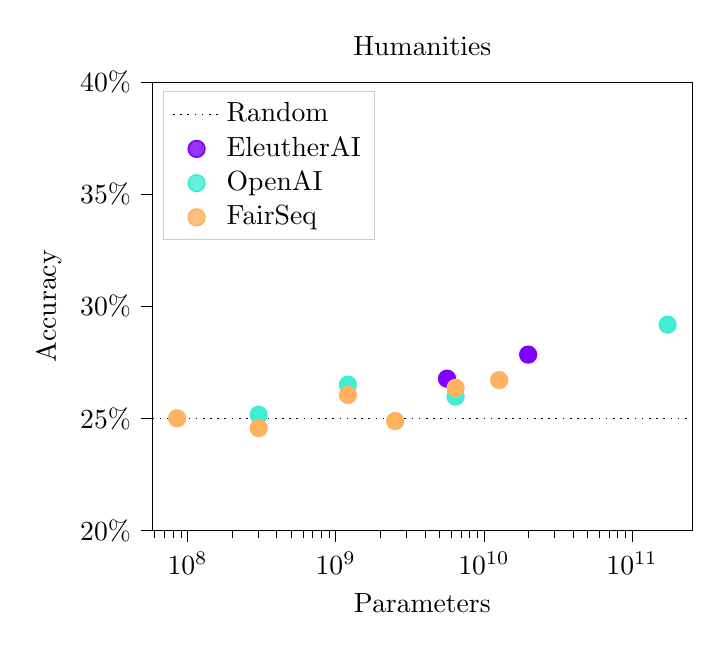
\begin{tikzpicture}

\definecolor{darkgray176}{RGB}{176,176,176}
\definecolor{darkviolet1270255}{RGB}{127,0,255}
\definecolor{lightgray204}{RGB}{204,204,204}
\definecolor{sandybrown25517896}{RGB}{255,178,96}
\definecolor{turquoise64236211}{RGB}{64,236,211}

\begin{axis}[
legend cell align={left},
legend style={fill opacity=0.8, draw opacity=1, text opacity=1, draw=lightgray204,at={(0.02,0.98)},anchor=north west},
log basis x={10},
tick align=outside,
tick pos=left,
title={Humanities},
x grid style={darkgray176},
xlabel={Parameters},
xmin=58012079.6447931, xmax=254672107396.429,
xmode=log,
xtick style={color=black},
y grid style={darkgray176},
ylabel={Accuracy},
ymin=0.2, ymax=0.4,
ytick style={color=black},
yticklabel={\pgfmathprintnumber{\tick}\%},
scaled y ticks=false,
y coord trafo/.code={\pgfmathparse{#1*100}\pgfmathresult}
]
\addplot [semithick, black, dotted]
table {%
58012079.644793 0.25
254672107396.429 0.25
};
\addlegendentry{Random}
\addplot [semithick, darkviolet1270255, mark=*, mark size=3, mark options={solid}, only marks]
table {%
5637144576 0.267738883632923
19900000000 0.27846105329549
};
\addlegendentry{EleutherAI}
\addplot [semithick, turquoise64236211, mark=*, mark size=3, mark options={solid}, only marks]
table {%
301989888 0.251647183846971
1207959552 0.265037194473964
6442450944 0.259723698193411
173946175488 0.291817215727949
};
\addlegendentry{OpenAI}
\addplot [semithick, sandybrown25517896, mark=*, mark size=3, mark options={solid}, only marks]
table {%
84934656 0.250078839482813
301989888 0.245663828445285
1207959552 0.260485651214128
2516582400 0.248817407757805
6442450944 0.263639230526648
12681408000 0.267108167770419
};
\addlegendentry{FairSeq}
\end{axis}

\end{tikzpicture}

        \phantomcaption\label{fig:hendrycks-humanities}
    \end{subfigure}
    \hfill
    \begin{subfigure}{0.49\textwidth}
        \centering
        % This file was created with tikzplotlib v0.10.1.
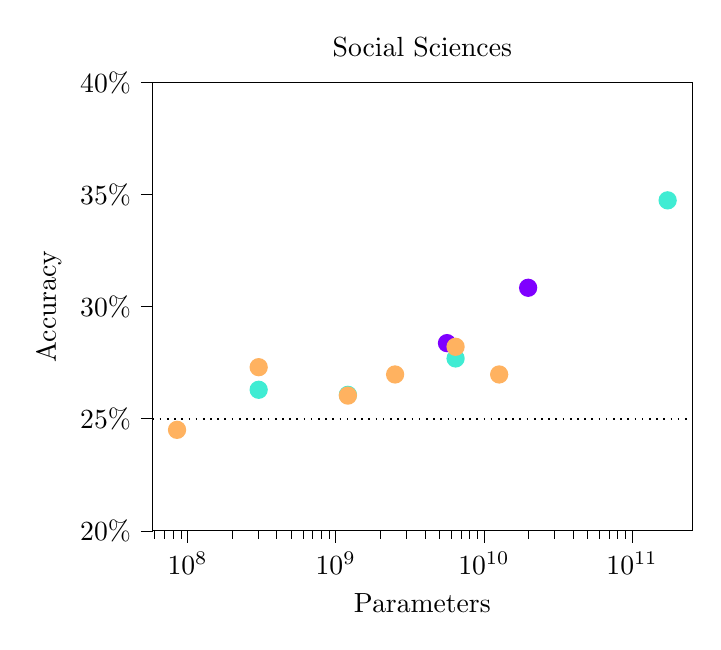
\begin{tikzpicture}

\definecolor{darkgray176}{RGB}{176,176,176}
\definecolor{darkviolet1270255}{RGB}{127,0,255}
\definecolor{lightgray204}{RGB}{204,204,204}
\definecolor{sandybrown25517896}{RGB}{255,178,96}
\definecolor{turquoise64236211}{RGB}{64,236,211}

\begin{axis}[
legend cell align={left},
legend style={fill opacity=0.8, draw opacity=1, text opacity=1, draw=lightgray204,at={(0.02,0.98)},anchor=north west},
log basis x={10},
tick align=outside,
tick pos=left,
title={Social Sciences},
x grid style={darkgray176},
xlabel={Parameters},
xmin=58012079.6447931, xmax=254672107396.429,
xmode=log,
xtick style={color=black},
y grid style={darkgray176},
ylabel={Accuracy},
ymin=0.2, ymax=0.4,
ytick style={color=black},
yticklabel={\pgfmathprintnumber{\tick}\%},
scaled y ticks=false,
y coord trafo/.code={\pgfmathparse{#1*100}\pgfmathresult}
]

\addplot [semithick, black, dotted]
table {%
58012079.644793 0.25
254672107396.429 0.25
};
%\addlegendentry{Random}
\addplot [semithick, darkviolet1270255, mark=*, mark size=3, mark options={solid}, only marks]
table {%
5637144576 0.283717907052324
19900000000 0.308417289567761
};
%\addlegendentry{EleutherAI}
\addplot [semithick, turquoise64236211, mark=*, mark size=3, mark options={solid}, only marks]
table {%
301989888 0.262918427039324
1207959552 0.260643483912902
6442450944 0.276893077673058
173946175488 0.347416314592135
};
%\addlegendentry{OpenAI}
\addplot [semithick, sandybrown25517896, mark=*, mark size=3, mark options={solid}, only marks]
table {%
84934656 0.245043873903152
301989888 0.272993175170621
1207959552 0.260318492037699
2516582400 0.26974325641859
6442450944 0.282092947676308
12681408000 0.26974325641859
};
%\addlegendentry{FairSeq}
\end{axis}

\end{tikzpicture}

    \end{subfigure}
    \vskip\baselineskip
    \begin{subfigure}{0.49\textwidth}
        \centering
        % This file was created with tikzplotlib v0.10.1.
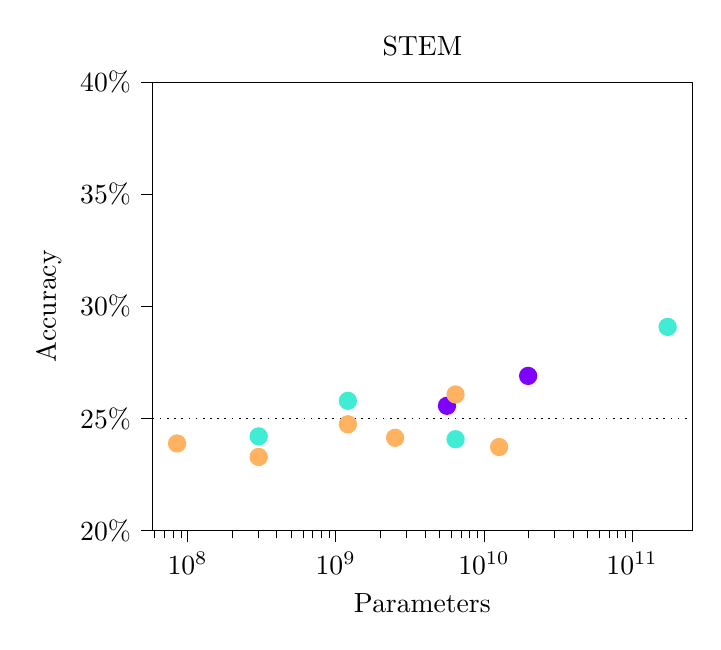
\begin{tikzpicture}

\definecolor{darkgray176}{RGB}{176,176,176}
\definecolor{darkviolet1270255}{RGB}{127,0,255}
\definecolor{lightgray204}{RGB}{204,204,204}
\definecolor{sandybrown25517896}{RGB}{255,178,96}
\definecolor{turquoise64236211}{RGB}{64,236,211}

\begin{axis}[
legend cell align={left},
legend style={fill opacity=0.8, draw opacity=1, text opacity=1, draw=lightgray204,at={(0.02,0.98)},anchor=north west},
log basis x={10},
tick align=outside,
tick pos=left,
title={STEM},
x grid style={darkgray176},
xlabel={Parameters},
xmin=58012079.6447931, xmax=254672107396.429,
xmode=log,
xtick style={color=black},
y grid style={darkgray176},
ylabel={Accuracy},
ymin=0.2, ymax=0.4,
ytick style={color=black},
yticklabel={\pgfmathprintnumber{\tick}\%},
scaled y ticks=false,
y coord trafo/.code={\pgfmathparse{#1*100}\pgfmathresult}
]

\addplot [semithick, black, dotted]
table {%
58012079.644793 0.25
254672107396.429 0.25
};
%\addlegendentry{Random}
\addplot [semithick, darkviolet1270255, mark=*, mark size=3, mark options={solid}, only marks]
table {%
5637144576 0.255629559150016
19900000000 0.268965517241379
};
%\addlegendentry{EleutherAI}
\addplot [semithick, turquoise64236211, mark=*, mark size=3, mark options={solid}, only marks]
table {%
301989888 0.241991753885189
1207959552 0.257849666983825
6442450944 0.240723120837298
173946175488 0.290834126228988
};
%\addlegendentry{OpenAI}
\addplot [semithick, sandybrown25517896, mark=*, mark size=3, mark options={solid}, only marks]
table {%
84934656 0.238820171265461
301989888 0.23279416428798
1207959552 0.247383444338725
2516582400 0.241357437361243
6442450944 0.260704091341579
12681408000 0.237234379955598
};
%\addlegendentry{FairSeq}
\end{axis}

\end{tikzpicture}

    \end{subfigure}
    \hfill
    \begin{subfigure}{0.49\textwidth}
        \centering
        % This file was created with tikzplotlib v0.10.1.
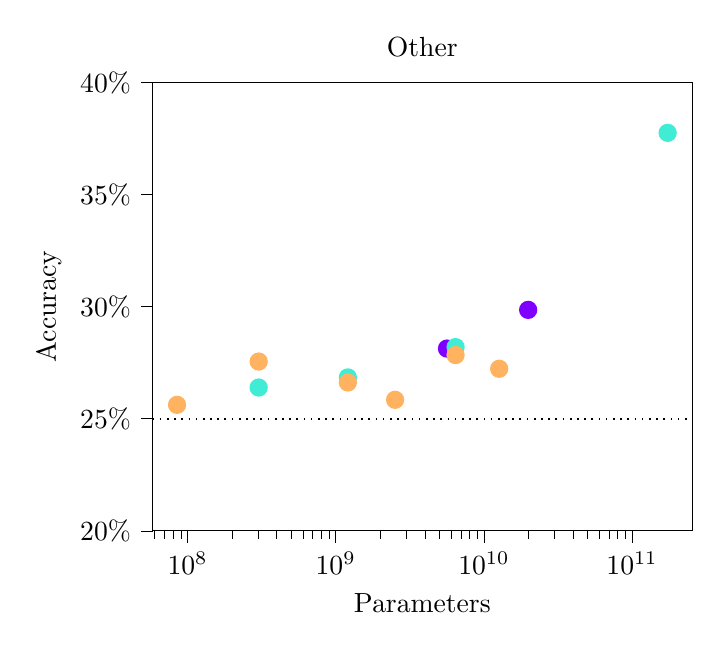
\begin{tikzpicture}

\definecolor{darkgray176}{RGB}{176,176,176}
\definecolor{darkviolet1270255}{RGB}{127,0,255}
\definecolor{lightgray204}{RGB}{204,204,204}
\definecolor{sandybrown25517896}{RGB}{255,178,96}
\definecolor{turquoise64236211}{RGB}{64,236,211}

\begin{axis}[
legend cell align={left},
legend style={fill opacity=0.8, draw opacity=1, text opacity=1, draw=lightgray204,at={(0.02,0.98)},anchor=north west},
log basis x={10},
tick align=outside,
tick pos=left,
title={Other},
x grid style={darkgray176},
xlabel={Parameters},
xmin=58012079.6447931, xmax=254672107396.429,
xmode=log,
xtick style={color=black},
y grid style={darkgray176},
ylabel={Accuracy},
ymin=0.2, ymax=0.4,
ytick style={color=black},
yticklabel={\pgfmathprintnumber{\tick}\%},
scaled y ticks=false,
y coord trafo/.code={\pgfmathparse{#1*100}\pgfmathresult}
]

\addplot [semithick, black, dotted]
table {%
58012079.644793 0.25
254672107396.429 0.25
};
%\addlegendentry{Random}
\addplot [semithick, darkviolet1270255, mark=*, mark size=3, mark options={solid}, only marks]
table {%
5637144576 0.28130028966849
19900000000 0.298559750875827
};
%\addlegendentry{EleutherAI}
\addplot [semithick, turquoise64236211, mark=*, mark size=3, mark options={solid}, only marks]
table {%
301989888 0.263920180238172
1207959552 0.268426134534921
6442450944 0.281943997425169
173946175488 0.377534599291922
};
%\addlegendentry{OpenAI}
\addplot [semithick, sandybrown25517896, mark=*, mark size=3, mark options={solid}, only marks]
table {%
84934656 0.25619568715803
301989888 0.275506919858384
1207959552 0.266173157386546
2516582400 0.258448664306405
6442450944 0.278403604763437
12681408000 0.272288381074992
};
%\addlegendentry{FairSeq}
\end{axis}

\end{tikzpicture}

    \end{subfigure}
    \caption{Zero-shot performance of \model{} and GPT-J-6B compared to FairSeq and OpenAI models on the Multitask Language Understanding dataset.}
\label{fig:hendrycks}
\end{figure}
\todo[inline]{make all the plots have lines}

\subsection{Mathematical Competency}

The solving of mathematical problems is an area that has had a long history of study in AI research. While large language models tend to perform quite poorly on both arithmetic tasks and mathematical problems phrased in natural language, there is growing evidence that this is primarily due to model design choices not considering this usecase carefully \citep{nogueira2021investigating}. We made two main choices aimed at improving performance on mathematical problems with GPT-NeoX: firstly, our tokenizer was created with mathematics in mind, and secondly a significant portion of our training data was mathematical texts in various forms (arXiv, DM Mathematics, Math Stack Exchange and Math Overflow).

To evaluate our success at creating a model that can succeed at mathematical tests we evaluate on the MATH test dataset \citep{hendrycks2021measuring}. Note that this is an evaluation metric that is designed to be finetuned on, but due to computational limitations we only evaluate models zero-shot here.

\begin{figure}
    \centering
    %\includegraphics{Figures/evals/plot_Math.png}
    \pgfplotsset{width=0.49\linewidth}
    % This file was created with tikzplotlib v0.10.1.
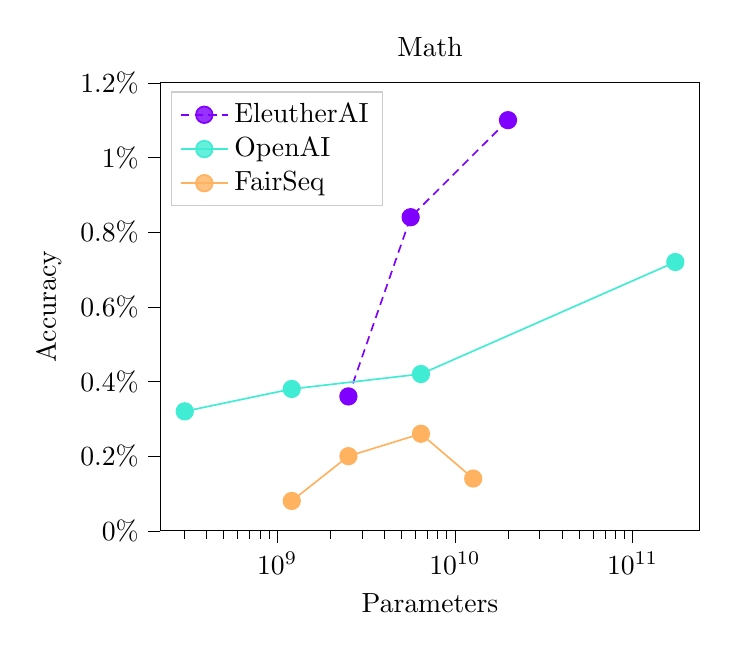
\begin{tikzpicture}

\definecolor{darkgray176}{RGB}{176,176,176}
\definecolor{darkviolet1270255}{RGB}{127,0,255}
\definecolor{lightgray204}{RGB}{204,204,204}
\definecolor{sandybrown25517896}{RGB}{255,178,96}
\definecolor{turquoise64236211}{RGB}{64,236,211}

\begin{axis}[
legend cell align={left},
legend style={fill opacity=0.8, draw opacity=1, text opacity=1, draw=lightgray204,at={(0.02,0.98)},anchor=north west},
log basis x={10},
tick align=outside,
tick pos=left,
title={Math},
x grid style={darkgray176},
xlabel={Parameters},
xmin=219771451.673039, xmax=239020972258.945,
xmode=log,
xtick style={color=black},
y grid style={darkgray176},
ylabel={Accuracy},
ymin=0, ymax=0.01201,
ytick style={color=black},
yticklabel={\pgfmathprintnumber{\tick}\%},
scaled y ticks=false,
y coord trafo/.code={\pgfmathparse{#1*100}\pgfmathresult}
]

\addplot [semithick, darkviolet1270255, mark=*, mark size=3, mark options={solid},densely dashed]
table {%
2516582400 0.0036
5637144576 0.0084
19900000000 0.011
};
\addlegendentry{EleutherAI}
\addplot [semithick, turquoise64236211, mark=*, mark size=3, mark options={solid}]
table {%
301989888 0.0032
1207959552 0.0038
6442450944 0.0042
173946175488 0.0072
};
\addlegendentry{OpenAI}
\addplot [semithick, sandybrown25517896, mark=*, mark size=3, mark options={solid}]
table {%
1207959552 0.0008
2516582400 0.002
6442450944 0.0026
12681408000 0.0014
};
\addlegendentry{FairSeq}
\end{axis}

\end{tikzpicture}

    \caption{Zero-shot performance of \model{}, GPT-J-6B, and GPT-Neo 2.7B compared to FairSeq and OpenAI models on the MATH dataset. Random performance on this task is $0\%$, and we were unable to find information on median human performance.}
    \label{fig:my_label}
\end{figure}
%\todo{fix y axis of MATH plot!! this 10^-2 thing is horrible and needs to go. also the legend is covering a point}

\todo[inline]{Eric to tikz-i-fy math plot and put it here}

As expected, all models perform extremely poorly on MATH in a zero-shot context. However, we find that \model{} is highly successful, relatively speaking, at this task and out-performs even GPT-3 175B. We also find that GPT-J, which was also trained on the Pile but doesn't have a mathematics-friendly tokenizer, matches GPT-3 175B's performance despite being 30x smaller. While we leave finetuning GPT-J and GPT-NeoX to future work, we view this as a strong indicator that pretraining on the Pile is an effective way to improve performance on mathematics tasks.

\section{Discussion}

Whilst the performance of the released 20B parameter model is impressive in many respects, outperforming our previous best performing model, GPT-J-6B, on most benchmarked datasets, it is clear from comparing to Fairseq's 13B parameter model \citep{fairseq-13B}, and extrapolating based on OpenAI's models' performance, that the performance on natural language tasks in particular could be improved, whilst the performance in other areas, such as scientific literature and mathematics excels. In this section we will try to dissect what the causes for these performance differences could be, and how we might be able to address them in future iterations. 

\textbf{Tokenizer and Dataset.} We expect some performance regression on web- and book-based language modeling benchmarks due to our tokenizer design favoring scientific and programming documents [Section \ref{sec:tokenization}] over web documents, as well as the former being much more prevalent in the Pile when compared to OpenAI's training set. However, it is not clear how to quantify the expected performance differences from these design choices.

\textbf{Hyperparameter Tuning.} Hyperparameter tuning is an expensive process, which for multi-billion parameter networks is often infeasible to do at full scale. Due to the aforementioned limitations, we opted to choose hyperparameters based on a mixture of experiments at smaller scales and by interpolating parameters appropriate for our model size based on previously published work \citep{brown2020language}. However, several aspects of both our model architecture [Section \ref{sec:model-arch}] and our training setup, including the data [Section \ref{sec:training-data}] and the tokenizer [Section \ref{sec:tokenization}], diverge significantly from \citet{brown2020language}. As such, it is almost certainly the case that the hyperparameters used for those models are no longer optimal, and potentially never were. 

The effects of certain hyperparameter choices on language models are sadly understudied, to the extent that many aspects of training large transformer models are effectively a folk art, only accessible to staff at a select number of private companies. For example, literature rigorously studying the effect of weight decay in language models is particularly scant \citep{fixnorm}, \citep{wd-reg}, and likewise, there is very little research investigating the effects of choices in designing a tokenizer---in particular the choice of vocabulary size---on downstream performance. 

It is possible that our choice of $0.01$ for weight decay was sub-optimal compared to GPT-3's choice of $0.1$, however, we note that Fairseq's recently released LMs \citep{fairseq-13B} also used a weight decay of $0.01$. Another possible source of performance regression could have been our choice of batch size. For efficiency reasons, we opted to use a fairly large batch size of 3.2M tokens during training, the same as was used by the 175B GPT-3 model. The critical batch size \citep{large-batch-training} for the model may have been lower, possibly resulting in a negative impact on training. In addition, the optimal learning rate---which we selected by interpolating between the learning rates for models in \citep{brown2020language}---can often be affected by the batch size, and failing to quantify this effect accurately could also have led to suboptimal performance. During the training of the model, however, new research has been released which may significantly alleviate the costs of hyperparameter tuning for future training runs \citep{yang2021tuning}.

\textbf{Dataset Deduplication.} Finally, the lack of dataset deduplication could also have had an impact on downstream performance. Recent research has shown that deduplicating training data can have a large effect on perplexity scores \citep{lee2021deduplicating}. Although GPT-J-6B was trained on the same data and performed on par with OpenAI's models of a similar size, it seems plausible that this effect could become particularly apparent with a larger model size.

\section{Broader Impacts}
\label{sec:broader-impacts}

We believe that Transformative Artificial Intelligence (TAI) \citep{tai} is approaching, and that these systems will cause catastrophic damage if they are misaligned with human values. As such, we believe it is essential to prioritize and help facilitate technical research that ensures TAI's values will be aligned with ours.

\textit{AI Alignment} generally refers to the problem of how to ensure increasingly powerful and autonomous AI systems perform the users' wishes faithfully and without unintended consequences. Alignment is especially critical as we approach human and superhuman levels of intelligence, as powerful optimization processes amplify small errors in goal specification into large misalignments \citep{Goodhart1984,Manheim2019Categorizing_Variants_of_Goodh}, and misalignments in this regime will result in runaway optimization processes that evade alteration or shutdown \citep{Omohundro2008TheBA,BensonTilsen2016FormalizingCI,turner2021optimal}, posing a significant existential risk to humanity. Additionally, even if the goal is specified correctly, superhuman models may still develop deceptive subsystems that attempt to influence the real world to satisfy their objectives \citep{hubinger2021rlo}. While current systems are not yet at the level where the consequences of misalignment pose an existential threat, rapid progress in the field of AI has increased the concern that the alignment problem may be seriously tested in the not-too-distant future.

Much of the alignment literature focuses on the more theoretical aspects of alignment \citep{demski2020embedded,yudkowsky2018functional,Taylor2016QuantilizersAS,Garrabrant2016LogicalI,Armstrong2018OccamsRI,hubinger2021rlo}, abstracting away the specifics of how intelligence will be implemented, due to uncertainty over the path to TAI. However, with the recent advances in capabilities, it may no longer be the case that the path to TAI is completely unpredictable. In particular, recent increases in the capabilities of large language models (LLMs) raises the possibility that the first generation of transformatively powerful AI systems may be based on similar principles and architectures as current large language models like GPT. This has motivated a number of research groups to work on “prosaic alignment” \citep{prosaic, askell2021general,instruct}, a field of study that considers the AI alignment problem in the case of TAI being built primarily with techniques already used in modern ML.
We believe that due to the speed of AI progress, there is a significant chance that this assumption is true, and, therefore, that contributing and enabling contributions to prosaic alignment research will have a large impact.

The open-source release of this model is motivated by the hope that it will allow alignment researchers who would not otherwise have access to LLMs to use them. While there are negative risks due to the potential acceleration of capabilities research, which may place further time pressure on solving the alignment problem, we believe the benefits of this release outweigh the risks of accelerating capabilities research.

\subsection{The Usefulness of Large Language Models in Alignment}

The alarming success of LLMs makes understanding them especially important for calibrating the theoretical and practical direction of alignment research. LLMs represent a different paradigm than the AI systems generally studied by alignment researchers because they are not well-described as coherent agents or expected utility maximizers. This introduces additional challenges, but also may enable new approaches to alignment. We briefly discuss some ways LLMs might be leveraged for alignment and some of the new problems they introduce below.

GPT-NeoX itself is not the system we need to align, but it can serve as a publicly available platform for experiments whose results might generalize to crucial future work. 

\subsubsection{Possible Approaches}

The following is a non-exhaustive list of potential approaches we consider promising for further investigation.\\

\textbf{Mechanistic interpretability.} Mechanistic interpretability research \citep{circuits} hopes to gain an understanding into \textit{how} models accomplish the tasks they do, in part in the hopes of detecting problematic or deceptive algorithms implemented by models before these failures manifest in the real world. Being able to interpret and inspect the detailed inner workings of trained models would be a powerful tool to ensure models are actually optimizing for the goals we intended \citep{hubinger2021rlo,koch2021objective}. Reverse engineering transformer language models has already yielded insights about the inner functioning of LMs \citep{anthropic-transformer-circuits,logit-lens, anonymous2022ROME, knowledge-neuron}. 

\textbf{Using a LLM as a reward model.} Because they learn to predict human writing, LLMs develop an extensive and nuanced embedding of human values at the semantic level. Finding a way to query those values is a possible path toward solving the problem of reward robustness in RL and other algorithms which require a proxy of human judgment \citep{rlhf-summ, alignment-by-default}. Despite fundamental theoretical limitations on learning human values \citep{Armstrong2018OccamsRI}, value learning may still be good enough for aligning weaker superhuman AIs. Future experiments could explore the extent to which LLM pretraining improves downstream reward model robustness and generalization.

\textbf{Natural language transparency.} Since LLM prompts are in a human-readable form, it can provide insight on the LLM’s expected behavior. Prompt programming or finetuning can be used to leverage this fact and force a LLM to execute more transparent algorithms, such as splitting problems into steps or explicitly writing an “internal monologue” \citep{visible-thoughts, factored-cognition}. Reliability and trustworthiness can present significant challenges for these approaches. 

However, this form of transparency also has its limits. In particular, models can often respond unpredictably to prompts, and internal monologues may become completely detached from the model's decision making process if translating between the model's ontology and the human ontology is more complex than simply modeling human monologues \citep{elk}.

%There are a number of projects underway within EleutherAI working on better understanding the internals of LMs using our models and training infrastructure. [examples]

\textbf{Simulating agents at runtime.} Unlike policies trained with reinforcement learning, self-supervised LLMs are not optimized with respect to a reward function and do not act as expected utility maximizers. However, given an appropriate prompt (such as a story of a character working to achieve a goal), LLMs can predict and thus simulate an agent \citep{huang2022language}. Such simulated agents could potentially have preferable safety characteristics compared to RL-trained agents, as due to the fact that they are not optimized for the objective directly they may be less susceptible to overoptimization. 
\todo[inline]{for janus: add some stuff on "why is it useful to experiment with simulated agents?" i added half a sentence but just want your input -leo}

However, language model simulated agents also have their downsides. A language model has a different epistemic state than that of the agent it is simulating, leading to trajectories which correspondingly act as if variables outside the context window are known and determined \citep{shaking-the-foundation,bc-miscalibrated}. This leads the model to suffer from “delusions” or “hallucinations” \citep{Shuster2021RetrievalAR,liu2021tokenlevel,Maynez2020OnFA}, and results in simulated agents that act overconfident relative to the model's epistemic state.

\textbf{Tool AI and automated alignment research.} LMs can be used as relatively unagentic tools, such as Codex \citep{chen2021evaluating} acting as a coding assistant. Because pretrained LLMs are not directly optimized for the factual accuracy of their predictions, it is possible they avoid some of the traditional problems with tool or oracle AI \citep{Armstrong2012ThinkingIT}, such as the incentive to produce manipulative answers \citep{predictomatic}. Tool AI is not a long-term solution to the problem of alignment, but it could be used to assist alignment research or even automate large parts of it.
\todo[inline]{for janus: what are some ways LLMs can be used to speed up alignment?}


\subsection{Lack of Access}

Despite the importance of prosaic alignment research, lack of access to large models presents a barrier to the types of research that can be explored by the wider research community. Having access to large models as close to the cutting edge as possible is essential for many research questions. Though some research can extrapolate from smaller models using scaling laws \citep{kaplan2020scaling}, some capabilities emerge only as models scale, and performance on tasks can increase discontinuously \citep{brown2020language}. Simply put, there are many properties of TAI you cannot study with models which can barely form coherent sentences.

Because training large models requires a significant engineering and capital investment, such models are often out of reach for small labs and independent researchers. As it stands, only large organizations have access to the latest generation of powerful language models \citep{brown2020language, gopher, switch-transformer, lieber2021jurassic, WuDao, fairseq-13B}. The number of researchers focused primarily on alignment working at these labs is only in the dozens. 

Safety is often used as a justification for keeping model weights closed-source. In practice, however, this is insufficient to prevent misuse. The public can already generate text using large language models through an increasing number of paid APIs provided by large corporations. As it stands, close-sourced models are primarily a limitation on the public’s ability to probe and modify large models. Though some types of prosaic alignment research can be done using only inference through an API, many require direct access to network weights. For example, interpretability research relies heavily on the ability to inspect and modify weights and activations, and many approaches to control and robustness require additional training. 

If only a small number of organizations and individuals have knowledge, access, and opportunity to work on pressing prosaic alignment problems, we are much more likely to fail. By openly training and releasing our large models, we hope to make it possible for more researchers to contribute to prosaic alignment. There are already a number of researchers using our previous models for alignment research \citep{logit-lens,anonymous2022ROME, lin2021truthfulqa}, and there are multiple RFPs requesting more [cite OpenPhil RFP, Beth Barnes RFP]
\todo[inline]{cite rfps}
\subsection{Impact on Capabilities Research}

Alignment is, in a sense, ``philosophy with a deadline'' \citep{superintelligence}. Given the rapid progress of AI Capabilities, it seems likely that we have limited time to solve the alignment problem before existentially dangerous AI systems are developed. As it stands, alignment research lags far behind capabilities research and does not seem likely to catch up if the current rates of progress continue.

Given that it seems infeasible to halt all AI capabilities research, we reason that focusing on work that advances the field of alignment more than it advances AI capabilities should provide a net reduction to existential risk. We feel the risk of releasing \model{} is acceptable, as the contribution of the model to capabilities research is likely to be limited, for two reasons. Firstly, the organizations pursuing capabilities research most aggressively are unlikely to benefit from our open-source release of this model because it significantly trails the state of the art. Second, we believe the single most impactful piece of knowledge that LLM research has had on advancing capabilities is the knowledge that scaling LMs was possible in the first place \citep{why-release}, whereas the actual implementation is very fungible (as evidenced by the large number of parties who have succeeded in creating their own LLMs).

We ultimately believe that the benefits of releasing this model outweigh the risks, but this argument hinges crucially on the particular circumstances of this release. All actors considering releasing powerful AI models or advancing the frontier of capabilities should think carefully about what they release, in what way, and when. 

\section{Summary}

We released \model{}, a 20 billion parameter auto-regressive transformer language model trained on the Pile \citep{gao2020pile} dataset, and detailed the main architectural differences between \model{} and GPT-3---most notably the change in tokenizer, the addition of Rotary embeddings, the parallel computation of attention and feed-forward layers, and a different initialization scheme and hyperparameters. We ran extensive evaluations of \model{} on natural language and factual knowledge tasks, and compared it with other publicly available models, finding it performed particularly well on knowledge-based and mathematical tasks. Finally, we are open sourcing the training and evaluation code at \url{https://github.com/EleutherAI/gpt-neox}, where you can also find a link to download the model weights across the whole training run.

\section*{Acknowledgments}

The authors would like to thank staff at CoreWeave---in particular Max~Hjelm, Brannin~McBee, Peter~Salanki and Brian~Venturo---for providing the GPUs and compute infrastructure that made this project possible, as well as Anthony~DiPofi, Charles~Foster, Jeffrey~Hsu, Eric~Tang, Anish~Thite, Kevin~Wang and Andy~Zou for their contributions to the EleutherAI Language Modeling Evaluation Harness, which we used to evaluate \model{}. 

The authors would also like to acknowledge Eren~Dogan and Wesley~Brown for feedback and technical support throughout the project, and John~Schulman and Evan~Hubinger for providing feedback on drafts of the paper.

\bibliography{citations}
\bibliographystyle{plainnat}

\appendix

\section{Individual Contributions}\label{app:contrib}

\textbf{Sid Black} was the lead developer and overall point person for the project. \textbf{Stella Biderman} was the project manager and led the scientific experimentation.


\paragraph{Implementation and Engineering:}
\begin{adjustwidth}{0.5cm}{}
\textbf{Implementation of training infrastructure:} Sid Black, Stella Biderman, Eric Hallahan, Quentin Anthony, Samuel Weinbach\\
\textbf{Scaling experiments and optimization:} Sid Black, Stella Biderman, Quentin Anthony, Samuel Weinbach\\
\textbf{Positional Embeddings:} Sid Black, Eric Hallahan, Michael Pieler\\
\textbf{Tokenizer:} Sid Black\\
\textbf{Misc:} USVSN Sai Prashanth, Ben Wang\\
\end{adjustwidth}

\paragraph{Scientific Experimentation:}
\begin{adjustwidth}{0.5cm}{}
\textbf{Evaluations:} Stella Biderman, Leo Gao, Jonathan Tow, Sid Black, Shivanshu Purohit, Horace He, Laurence Golding\\
\textbf{Positional Embeddings} Stella Biderman, Laurence Golding, Michael Pieler\\
\textbf{Tokenizer:} Stella Biderman, Jason Phang, Leo Gao\\
\end{adjustwidth}

\paragraph{Broader Impacts}
\begin{adjustwidth}{0.5cm}{}
\textbf{Alignment Implications:} Leo Gao, Connor Leahy, Laria Reynolds, Kyle McDonell
\end{adjustwidth}

\section{Full Configuration Details}\label{app:hparam}

In Table \ref{tab:config} we attach the full configuration details used to train \model{}. The file is available in .yaml format usable in gpt-neox at \url{https://github.com/EleutherAI/gpt-neox}, where you can also access documentation describing the role of each parameter.

\begin{table}[ht!]
\small
\centering
\begin{subtable}[h]{0.48\textwidth}
\begin{tabular}{lrrcc}
\hline
Configuration Key                               & Value \\
\hline
    attention-dropout & 0 \\
    bias-gelu-fusion & True \\
    checkpoint-activations & True \\
    checkpoint-num-layers & 1 \\
    data-impl & mmap \\
    distributed-backend & nccl \\
    eval-interval & 1000 \\
    eval-iters & 10 \\
    fp16.enabled & True \\
    fp16.fp16 & True \\
    fp16.hysteresis & 2 \\
    fp16.initial-scale-power & 12 \\
    fp16.loss-scale & 0 \\
    fp16.loss-scale-window & 1000 \\
    fp16.min-loss-scale & 1 \\
    gpt-j-residual & True \\
    gradient-accumulation-steps & 32 \\
    gradient-clipping & 1.0 \\
    hidden-dropout & 0 \\
    hidden-size & 6144 \\
    init-method & small-init \\
    log-interval & 2 \\
    lr-decay-iters & 150000 \\
    lr-decay-style & cosine \\
    max-position-embeddings & 2048 \\
    min-lr & 9.7e-06 \\
    model-parallel-size & 2 \\
    no-weight-tying & True \\
    norm & layernorm \\
    num-attention-heads & 64 \\
    num-layers & 44 \\
\end{tabular}

\end{subtable}
\begin{subtable}[h]{0.48\textwidth}
\begin{tabular}{lrrcc}
\hline
Configuration Key                               & Value \\
\hline
    optimizer.params.betas & [0.9, 0.95] \\
    optimizer.params.eps & 1e-08 \\
    optimizer.params.lr & 9.7e-05 \\
    optimizer.type & Adam \\
    output-layer-init-method & wang-init \\
    output-layer-parallelism & column \\
    partition-activations & False \\
    pipe-parallel-size & 4 \\
    pos-emb & rotary \\
    rotary-pct & 0.25 \\
    save-interval & 500 \\
    scaled-upper-triang-masked-softmax-fusion & True \\
    seq-length & 2048 \\
    split & 995,4,1 \\
    steps-per-print & 2 \\
    synchronize-each-layer & True \\
    tokenizer-type & HFTokenizer \\
    train-iters & 150000 \\
    train-micro-batch-size-per-gpu & 4 \\
    vocab-file & 20B-tokenizer.json \\
    wall-clock-breakdown & False \\
    warmup & 0.01 \\
    weight-decay & 0.01 \\
    zero-optimization.allgather-bucket-size & 1260000000 \\
    zero-optimization.allgather-partitions & True \\
    zero-optimization.contiguous-gradients & True \\
    zero-optimization.cpu-offload & False \\
    zero-optimization.overlap-comm & True \\
    zero-optimization.reduce-bucket-size & 1260000000 \\
    zero-optimization.reduce-scatter & True \\
    zero-optimization.stage & 1 \\
    \end{tabular}
\end{subtable}
\caption{The full configuration details for \model{} training}
\label{tab:config}
\end{table}

\section{Full Evaluation Results}\label{app:downstream}

\section{Model Card}\label{app:model-card}

%\section{Data Leakage Evaluation}\label{app:leakage}

\section{Tokenization Examples}\label{app:tokenization}

\begin{figure}[h]
    \centering
    \includegraphics[width=0.95\textwidth]{Figures/tokenization/examples/ArXiv.png}
    \caption{Pile (ArXiv) Tokenization Example}
    \label{fig:tok_example_0}
\end{figure}

\begin{figure}[h]
    \centering
    \includegraphics[width=0.95\textwidth]{Figures/tokenization/examples/BookCorpus2.png}
    \caption{Pile (BookCorpus2) Tokenization Example}
    \label{fig:tok_example_1}
\end{figure}

\begin{figure}[h]
    \centering
    \includegraphics[width=0.95\textwidth]{Figures/tokenization/examples/Books3.png}
    \caption{Pile (Books3) Tokenization Example}
    \label{fig:tok_example_2}
\end{figure}

\begin{figure}[h]
    \centering
    \includegraphics[width=0.95\textwidth]{Figures/tokenization/examples/DM Mathematics.png}
    \caption{Pile (DM Mathematics) Tokenization Example}
    \label{fig:tok_example_3}
\end{figure}

\begin{figure}[h]
    \centering
    \includegraphics[width=0.95\textwidth]{Figures/tokenization/examples/Enron Emails.png}
    \caption{Pile (Enron Emails) Tokenization Example}
    \label{fig:tok_example_4}
\end{figure}

\begin{figure}[h]
    \centering
    \includegraphics[width=0.95\textwidth]{Figures/tokenization/examples/EuroParl.png}
    \caption{Pile (EuroParl) Tokenization Example}
    \label{fig:tok_example_5}
\end{figure}

\begin{figure}[h]
    \centering
    \includegraphics[width=0.95\textwidth]{Figures/tokenization/examples/FreeLaw.png}
    \caption{Pile (FreeLaw) Tokenization Example}
    \label{fig:tok_example_6}
\end{figure}

\begin{figure}[h]
    \centering
    \includegraphics[width=0.95\textwidth]{Figures/tokenization/examples/Github.png}
    \caption{Pile (Github) Tokenization Example}
    \label{fig:tok_example_7}
\end{figure}

\begin{figure}[h]
    \centering
    \includegraphics[width=0.95\textwidth]{Figures/tokenization/examples/Gutenberg (PG-19).png}
    \caption{Pile (Gutenberg (PG-19)) Tokenization Example}
    \label{fig:tok_example_8}
\end{figure}

\begin{figure}[h]
    \centering
    \includegraphics[width=0.95\textwidth]{Figures/tokenization/examples/HackerNews.png}
    \caption{Pile (HackerNews) Tokenization Example}
    \label{fig:tok_example_9}
\end{figure}

\begin{figure}[h]
    \centering
    \includegraphics[width=0.95\textwidth]{Figures/tokenization/examples/NIH ExPorter.png}
    \caption{Pile (NIH ExPorter) Tokenization Example}
    \label{fig:tok_example_10}
\end{figure}

\begin{figure}[h]
    \centering
    \includegraphics[width=0.95\textwidth]{Figures/tokenization/examples/OpenSubtitles.png}
    \caption{Pile (OpenSubtitles) Tokenization Example}
    \label{fig:tok_example_11}
\end{figure}

\begin{figure}[h]
    \centering
    \includegraphics[width=0.95\textwidth]{Figures/tokenization/examples/OpenWebText2.png}
    \caption{Pile (OpenWebText2) Tokenization Example}
    \label{fig:tok_example_12}
\end{figure}

\begin{figure}[h]
    \centering
    \includegraphics[width=0.95\textwidth]{Figures/tokenization/examples/PhilPapers.png}
    \caption{Pile (PhilPapers) Tokenization Example}
    \label{fig:tok_example_13}
\end{figure}

\begin{figure}[h]
    \centering
    \includegraphics[width=0.95\textwidth]{Figures/tokenization/examples/Pile-CC.png}
    \caption{Pile (Pile-CC) Tokenization Example}
    \label{fig:tok_example_14}
\end{figure}

\begin{figure}[h]
    \centering
    \includegraphics[width=0.95\textwidth]{Figures/tokenization/examples/PubMed Abstracts.png}
    \caption{Pile (PubMed Abstracts) Tokenization Example}
    \label{fig:tok_example_15}
\end{figure}

\begin{figure}[h]
    \centering
    \includegraphics[width=0.95\textwidth]{Figures/tokenization/examples/PubMed Central.png}
    \caption{Pile (PubMed Central) Tokenization Example}
    \label{fig:tok_example_16}
\end{figure}

\begin{figure}[h]
    \centering
    \includegraphics[width=0.95\textwidth]{Figures/tokenization/examples/StackExchange.png}
    \caption{Pile (StackExchange) Tokenization Example}
    \label{fig:tok_example_17}
\end{figure}

\begin{figure}[h]
    \centering
    \includegraphics[width=0.95\textwidth]{Figures/tokenization/examples/USPTO Backgrounds.png}
    \caption{Pile (USPTO Backgrounds) Tokenization Example}
    \label{fig:tok_example_18}
\end{figure}

\begin{figure}[h]
    \centering
    \includegraphics[width=0.95\textwidth]{Figures/tokenization/examples/Ubuntu IRC.png}
    \caption{Pile (Ubuntu IRC) Tokenization Example}
    \label{fig:tok_example_19}
\end{figure}

\begin{figure}[h]
    \centering
    \includegraphics[width=0.95\textwidth]{Figures/tokenization/examples/Wikipedia (en).png}
    \caption{Pile (Wikipedia (en)) Tokenization Example}
    \label{fig:tok_example_20}
\end{figure}

\begin{figure}[h]
    \centering
    \includegraphics[width=0.95\textwidth]{Figures/tokenization/examples/YoutubeSubtitles.png}
    \caption{Pile (YoutubeSubtitles) Tokenization Example}
    \label{fig:tok_example_21}
\end{figure}


\end{document}